%% nicht vergessen draft raus zu nehmen, um echte Bilder einzubinden und die Problem-Vierecke verschwinden zu lassen
\documentclass[11pt,a4paper,oneside,svgnames]{report}

\usepackage[utf8]{inputenc}
\usepackage[T1]{fontenc}
\usepackage{lmodern}
\usepackage{eurosym}
\usepackage[british]{babel}
\usepackage{float}

\usepackage{longtable}
\usepackage{ae}
\usepackage{hyperref}
\usepackage[table]{xcolor}
\usepackage{colortbl}
\usepackage{multirow}
\usepackage{tabularx}
\usepackage{graphicx}
\usepackage{tikz}
\usepackage{kpfonts}
\usepackage[explicit]{titlesec}
\usepackage[acronym,nonumberlist,style=tree]{glossaries}
\usepackage{amssymb}
\usepackage[left=3.65cm,right=3.65cm]{geometry}
\usepackage{listings}


%BEGIN Chapter Definition

\makeatletter
\def\thickhrulefill{\leavevmode \leaders \hrule height 1ex \hfill \kern \z@}
\def\@makechapterhead#1{%
  \vspace*{10\p@}%
  {\parindent \z@ \raggedleft \reset@font
            \scshape \@chapapp{} \thechapter
        \par\nobreak
        \interlinepenalty\@M
    \Huge \bfseries #1\par\nobreak
    %\vspace*{1\p@}%
    \hrulefill
    \par\nobreak
    \vskip 50\p@
  }}
\def\@makeschapterhead#1{%
  \vspace*{10\p@}%
  {\parindent \z@ \raggedleft \reset@font
            \scshape \vphantom{\@chapapp{} \thechapter}
        \par\nobreak
        \interlinepenalty\@M
    \Huge \bfseries #1\par\nobreak
    %\vspace*{1\p@}%
    \hrulefill
    \par\nobreak
    \vskip 50\p@
  }}

%END Chapter Definition

%BEGIN Title Definition

\makeatletter
\def\thickhrulefill{\leavevmode \leaders \hrule height 1pt\hfill \kern \z@}
\renewcommand{\maketitle}{\begin{titlepage}%
    \let\footnotesize\small
    \let\footnoterule\relax
    \parindent \z@
    \reset@font
    \null\vfil
    \begin{flushleft}
      \huge \@title
    \end{flushleft}
    \par
    \hrule height 4pt
    \par
    \begin{flushright}
      \LARGE \@author \par
    \end{flushright}
    \vskip 60\p@
    \vfil\null
  \end{titlepage}%
  \setcounter{footnote}{0}%
}

%END Title Definition

%Verschissener rotierter Text für verschissene Tabelle 14.1/2
\makeatletter
\newsavebox\zzz
\def\mystrut{%
\dimen@\wd\zzz
\divide\dimen@\thr@@
\advance\dimen@-\dp\@arstrutbox
\rule\z@\dimen@}

\def\rotatezzz{%
\rotatebox{90}{\rlap{\kern-\dp\@arstrutbox\usebox\zzz}}}
%END Verschissener rotierter Text

\makeatother
\title{Structured Design for Project ``BookExpress''}
\author{Marc A. Harnos\\ {mharnos@gmail.com} \and Joscha Rapp\\ {jraxxo@gmail.com} \and Christian Schulz\\ {crs.s@gmx.net}}
\author{Marc A. Harnos\\ Joscha Rapp\\ Christian Schulz}
\date{October 2012}

\definecolor{tableHead}{HTML}{5393B7}
\definecolor{tableEven}{HTML}{DAF1FF}
\definecolor{tableOdd}{HTML}{ADD0E5}
\definecolor{tableFoot}{HTML}{5393B7}

\definecolor{linkcolour}{rgb}{0,0.2,0.6}

\hypersetup{colorlinks,breaklinks,urlcolor=linkcolour,linkcolor=linkcolour}
\renewcommand{\arraystretch}{1.25}

\makeglossaries

\newglossaryentry{mvc}{name=MVC,description={Model View Controller},plural=MVCs, first={Model View Controller (MVC)}}

\newglossaryentry{jsp}{name=JSP,description={Java Server Page},plural=JSPs, first={Java Server Page (JSP)}, firstplural={Java Server Pages (JSPs)}}

\newglossaryentry{jre}{name=JRE,description={Java Runtime Environment},plural=JRE, first={Java Runtime Environment (JRE)}}

\newglossaryentry{jvm}{name=JVM,description={Java Virtual Machine},plural=JVM, first={Java Virtual Machine (JVM)}}

\newacronym{led}{LED}{light-emitting diode}


\begin{document}

\maketitle
\tableofcontents

\chapter*{Document History}

\begin{table}[H]
\centering
\begin{tabular}{|p{3.8cm}|p{2cm}|p{5.5cm}|p{1.2cm}|}
\hline 
Editor(s) & Date & Purpose of Editing & Version \\ 
\hline 
Schulz & 2012-10-05 & Initial Document Creation, add Introduction and Environment till Database Server & v0.1 \\ 
\hline
Harnos, Rapp & 2012-10-06 & Added leftover Environment and Software Architecture & v0.2 \\ 
\hline
Rapp & 2012-10-07 & Added some Software Modules and updated Environment & v0.4 \\ 
\hline 
Harnos, Rapp, Schulz & 2012-10-11 & Added Data Dictionary and updated Model Layers diagram & v0.5 \\ 
\hline
Harnos & 2012-10-13 & General Architecture and added missing Software Modules  & v0.6 \\ 
\hline 
Rapp, Schulz & 2012-10-18 & Added Mini Specifications & v0.9\\ 
\hline
Harnos, Rapp, Schulz & 2012-10-21 & Final check for spelling and correctness & v1.0\\ 
\hline 
\end{tabular}
\caption{Document History Table}
\label{tab:document-history}
\end{table}


\chapter{Introduction}
This structured design gives a detailed overview of the software design and system architecture, based on the previously developed requirement analysis and structured analysis. The structured design should be later on used for the implementation of the "BookExpress" system.

This document describes the specifications for the software architecture, the functional abstraction layer of the previously defined data flow diagrams and detailed specification of the system modules.

The description of the specific modules will vary in abstraction, allowing the software architect to implement his own, or the companies preferred, standards, without interfering in product functionality; whenever necessary the definitions provided will be more granular ensuring consistent quality and enforcing expected behaviour.

Some description will have overlapping information with the requirements specification, in case this document is sent stand alone, to assure all information is being provided.

\chapter{Environment / General~Architecture}
This chapter describes the general architecture of the system and the environment, general information will be provided for the system here, which will be described in the next chapter in depth; also detailed hardware and software specifications will be discussed in this chapter.

\begin{figure}[H]
 \begin{center}
  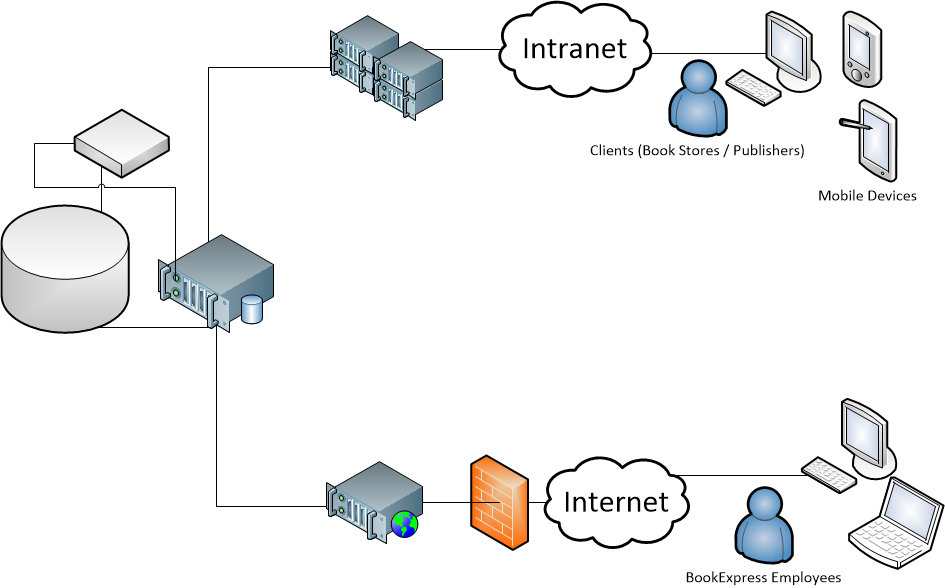
\includegraphics[width=\textwidth]{Hardware Structure.png}
 \end{center}
 \caption{Hardware Structure}
\end{figure}

\section{Application Server}
The application server incorporates the business logic and database requests and queries. It provides the business and data access layer of the application which is described in \ref{sec:mvc-pattern}. The application server processes requests from the web server and makes data objects in response to those requests, which can be used by the web server.

\section{Web Server}
The web server is implemented as a separate Java web server, like Tomcat, which can be incorporated in the application server, but also can run stand alone on another server. The server only processes requests from the web interface and decides which page to show, or if data received can be stored.

The web server is only accessible through a certain range of ports which are necessary to display standard web pages and secure web pages, to prevent hijacking or the manipulation of server configuration files.

\section{Database Server}
The database server provides any data requested from the application server and can be hosted on separate servers, but could also be on the same hardware infrastructure. The server should be an advanced and stable system like an IBM DB2 System or an Oracle Database Management System, a MySql solution might also be applicable, but the better performance, faster response times and stability of dedicated database systems would be preferable.

\section{Server Environment}
For the product to work, servers must be able to run the \gls{jvm} on which our Java application server runs. The server could be any type of mainframe with virtualisation technology; but also any type of individual Unix or Windows servers with the server applications physically separate.

An Unix system is preferable for the fewer system load from the operating system and improved stability. The data storage could also be allocated on separate storage units like medium sized magnetic storage units from IBM or HP.

The important part is, that the servers have at least this kind of specification for the individual servers, the application server, web server and database server, or cumulative on big servers or mainframes:

\begin{itemize}
	\item at least 4GHz Quad-Core CPU per server
	\item for each server at least 12 GB of RAM, for the database server at least 32GB
	\item enough storage for temporary files and data, at least 1-3 TB per server, and at least 3-5TB for the application server
\end{itemize}

A fast LAN connection is required for each server; this connection should at least be a 10GBit connection so servers in a server farm or computing centre communicate as fast as possible minimizing data retrieval times.

\section{Client Environment}
\subsection{Hardware}
The hardware specifications for the client are basically the minimal requirements of the operating system. The client also should not have less than 2GB of RAM.

Also the machine has to be able to access the network via an ethernet adapter so information from the web server application can be retrieved. The client's machine has to have enough free usb ports to support additional hardware like the graphical tablet, bar code readers and other possible hardware additions to the stand alone client.
\subsection{Software}
\subsubsection{Web Interface}
The web interface is accessed through a web browser - this browser should be standards compliant.

This list shows the supported browsers, but any other browser can work too, as long as it implements standards obedient rendering engines.

\begin{itemize}
	\item Firefox (version 3.5 or higher)
	\item Chrome (any version)
	\item Safari (version 4 or higher)
	\item Opera (version 9 or higher)
	\item Internet Explorer (version 10 or higher)
\end{itemize}
\subsubsection{Client Application}
The client application for "BookExpress" employees should have the \gls{jre} installed, so the application can be executed. The operating system does not matter, but some hardware could possibly not be accessed by certain operating system, therefore also drivers for special hardware add ons, like the previously mentioned tablets and bar code readers, should be installable and present.

\chapter{Software Architecture}
The software architecture of a system is the set of structures needed to reason about the system, which comprise software elements, relations among them, and properties of both. The term also refers to documentation of a system's "software architecture".\footnote{ Clements, Paul; Felix Bachmann, Len Bass, David Garlan, James Ivers, Reed Little, Paulo Merson, Robert Nord, Judith Stafford (2010). Documenting Software Architectures: Views and Beyond, Second Edition. Boston: Addison-Wesley. ISBN 0-321-55268-7.}\footnote{Bass, Len; Paul Clements, Rick Kazman (2012). Software Architecture In Practice, Third Edition. Boston: Addison-Wesley. pp. 25–37. ISBN 0-321-81573-4.}

In this chapter the programming pattern which the software architect has to implement is discussed at first, then common techniques for standardizing the code and enhancing readability and the used software and at last the implementation of the pattern into the software solution itself.

\section{Programming Pattern}
\label{sec:mvc-pattern}
The "BookExpress" software should implement a simple \gls{mvc} pattern separating the user visible output from the internal data processing structures much like CSS separates the styling of a webpage from the HTML markup.

The "Model" part of this set up fetches data from databases and holds them in objects - it is essentially the "data storage" of the application. The controller and view must not make any database queries, all data required for the specific controller/view has to be provided by the model itself, which in turn does make the necessary database requests. This can speed up the data retrieving process with smart caching times on the model part and also ensures a higher level of security by minimizing the chance of SQL-Injections possibly performed on the controller/view.

The "View" is essentially anything the user gets to see on his side of the application - the user interface. It also is the only point where the user can interact with the application, evaluating and providing data. The view itself can only retrieve data from the model, it can never make direct database lookups.

The "Controller" holds the business and processing logic of the software. It decides which view should be displayed to the user and which model could be used. Any data sent from the view/the user is processed by the controller and sent to the appropriate models.

In the "BookExpress" software there are two different implementations of this \gls{mvc} pattern. The web interface is the view component for the book shops and publishers, they interact with this view over their web browsers.
For this view, the controller is implemented on the application server as a web server, providing requested views and processing delivered input data. The communication between the view and controller is made over the standard network protocol tcp/ip and the data transmitted varies from standard HTML/text pages to compressed JSON data, for asynchronous and dynamic client view updates.

The "Model" in the first - and also in the second - set up is the application server itself, on which the web server runs. The application server is on the same machine as the web server, but logically a separate entity; it has access to the database server, which can also run on the same hardware, but also could run on a different machine. The data transmitted from model to controller and vice versa is composed of data objects transmitted binary for instant usage on the individual server; we do not have to compress data here, or serialize it, for the lack of data travelling distance.

In the second case, when the "BookExpress" employees use the client application software, the \gls{mvc} varies a bit from the web interface implementation. Here the application itself has its separate model, view and controller, which in turn all three act as a controller \textbf{and} view unit and the outlying model is on the application server in an different location. Therefore the data transmitted from this controller construct to the model and vice versa has to be compressed and serialized, utilizing JSON and gzip compression to accomplish fast serialisation and minimisation for faster response times and as little as possible data transferred. The communication between the inner model and inner controller are - as with the implementation on the application server - uncompressed and binary transferrals of Java objects.

This set up accomplishes that the inner model can cache data and minimize the needed look up to the model on the application server, where as the inner controller and view do not have to be modified for this "special environment"; they get their data as if they were directly connected to the outer model - but with enhanced performance.

\begin{figure}[H]
 \begin{center}
  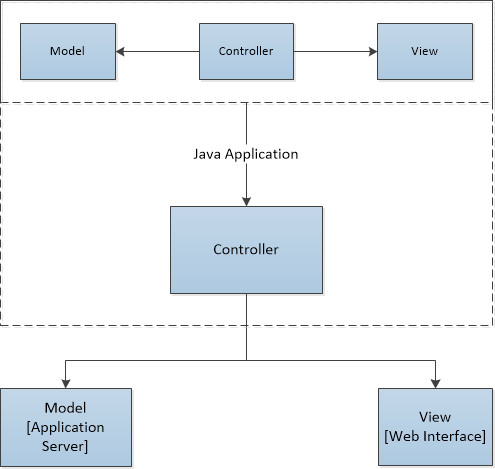
\includegraphics[width=\textwidth]{MVC-small.png}
 \end{center}
 \caption{MVC Pattern}
\end{figure}

\section{Programming Techniques and Software}
For standardisations and readabilities sake simple rules should be honoured to ensure a consistent look of program code, making it for new software architects joining the team easier to understand the code and find code parts faster. Those rules are arbitrary and should be agreed upon the development team; they should be defined at the beginning of the project and extended if necessary. An example for such a rule would be the placement of curly braces after method declarations, they could be defined directly after the declaration or in a new line.

\lstset{
	tabsize=4,
	rulecolor=,
	language=Java,
        basicstyle=\scriptsize,
        upquote=true,
        aboveskip={1.5\baselineskip},
        columns=fixed,
        showstringspaces=false,
        extendedchars=true,
        breaklines=true,
        prebreak = \raisebox{0ex}[0ex][0ex]{\ensuremath{\hookleftarrow}},
        frame=single,
        showtabs=false,
        showspaces=false,
        showstringspaces=false,
        identifierstyle=\ttfamily,
        keywordstyle=\color[rgb]{0,0,1},
        commentstyle=\color[rgb]{0.133,0.545,0.133},
        stringstyle=\color[rgb]{0.627,0.126,0.941},
        captionpos=b
}

\begin{lstlisting}[caption={Example of method declaration with curly braces in single and new line},label=javaCodeExampleCurlyBraces]
/*
 * Example for main method with curly braces directly 
 * after method declaration
 */
public static void main(String[] argv) {
	String where = "down below";
	System.out.println("Your code goes " + where);
}

/*
 * This main method declaration has the curly braces 
 * after a line break
 */
public static void main(String[] args)
{
	System.out.println("Your code goes here, maybe.");
}
\end{lstlisting}

The application server should be implemented with a Java application server; it does not matter if this server application is commercial or open source, as long as it is Sun/Oracle certified for Java EE application servers\footnote{http://www.oracle.com/technetwork/java/javaee/overview/compatibility-jsp-136984.html}.
The server could be a WebSphere Application Server from IBM, but also an TomEE from Apache, as long as it has all the required server modules for running a web server.

Java EE should be used due to a number of advantages:
\begin{itemize}
	\item Implementation of MVC pattern comes naturally with Java EE application servers, because of how Java in general works and in particular the application server is modelled with APIs and object oriented modularisation
	\item It is a very popular software used by many companies, so the chances that the implementing software architect has already experience with it is very likely
	\item The web server system is faster than common PHP servers, due to the compilation of web pages rather than script interpretation
\end{itemize}

For the database there is also the choice between a proprietary, commercial system like DB2 from IBM or an open source solution like a MySQL server; the important thing is, that the database supports standard SQL queries - not requiring the alteration of SQL statements/queries for the sake of proprietary solutions like special JOIN cases on some Microsoft database systems.

\section{Implementation}
\subsection{Data Storage/Application Server (Model)}
The model, which runs on the Java application server, has a intermediate connection to the database server and delivers the required information for the view and controller in form of Java Beans or JSON strings.

The model also has an implemented security layer, denying access to data, which the user has no privileges to and blocking malicious requests. This security layer has to work quick, and in general the model has to be very responsive, due to the high data load.

\subsection{Web Interface (View)}
The view is the point, the interaction between the book stores, publishers and the system takes place. The web interface should look the same on, and work with any new and standards compliant web browser; the supported browsers should at least include Mozilla Firefox from version 3.5 onwards, Chrome, Opera from version 9 onwards, Safari, and Internet Explorer from version 10 onwards.

The view itself should output standard complaint HTML5 code, and use modern JavaScript libraries to enhance the user experience and make user work flow easier to understand, i.e. by implementing visual clues which data is currently missing and suggesting search and input terms where appropriate.

The work flow has to be easy to understand, and the input fields and buttons should be recognised fast and placed on similar locations for each individual task, for faster learning curves and easy and fast pattern remembering.

\subsection{Application Server/Web Server (Controller)}
The controller is processing user data, which always implies input errors and the possibility of an attack to the system. The data has to be checked for any inconsistency regarding data type and for missing data - also any attempt of system intrusion has to be recognised and prevented.
The controller has a security and rights management layer implemented, preventing users from seeing views, they should not be able to see.

The controller is running on a web server and is realised through \glspl{jsp}.

\subsection{Client Application (Controller/View)}
The client application is a stand alone Java application which incorporates the model, view and controller into one program, and is regarded as a controller unit itself. The data is retrieved from the application server and transmitted serialised through JSON strings into the model of the application. Hereby security is very important, the data is never transmitted without encryption ensuring packages could not be sniffed over the network. The whole application as a controller has to be written so it cannot be manipulated in a form, where the user is given more rights than he actually has - without model authorisation the controller should not be able to process any data to the view nor retrieve such data from the model on the web server itself.

The client application should be very responsive and fast - it also should integrate in the system very well enabling features as drag\&drop and the support for specialised hardware like graphical tablets for signature processing and bar code readers or gps tracking devices.

\section{Model Layers}
\begin{figure}[H]
 \begin{center}
  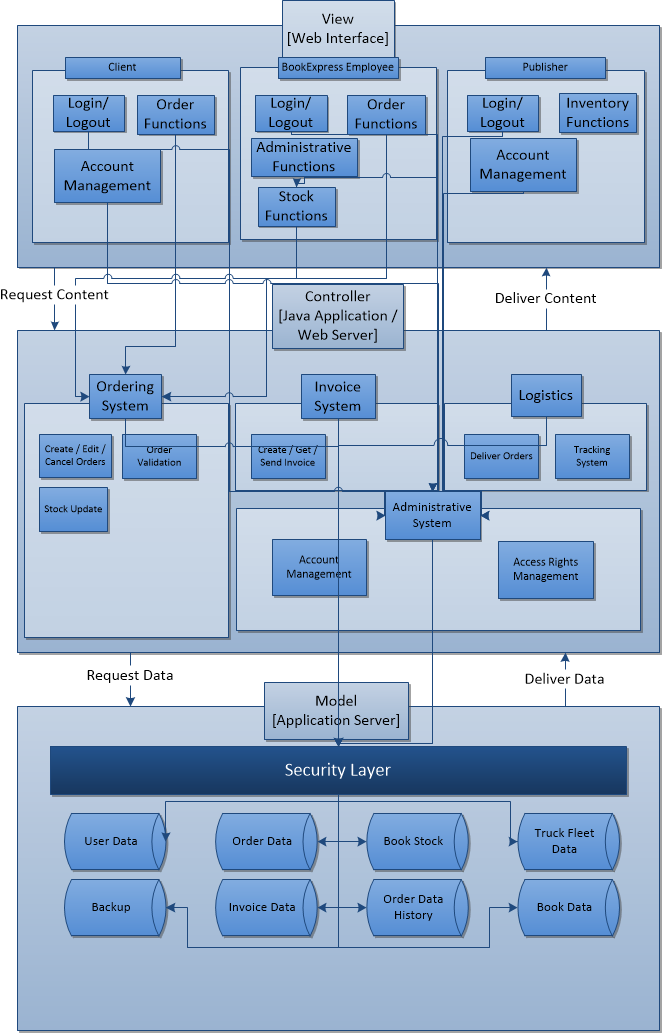
\includegraphics[width=\textwidth]{LayeredModel.png}
 \end{center}
 \caption{Model Layers}
\end{figure}

The figure describes the MVC patttern for BookExpress and consist of a View (Web Interface), Controller (Java Application / Web Server) and Model (Application Server).

As shown in the diagram, the Client, Publisher and BookExpress Employees all use the same Web Interface to process data and functions but have different rights as to the different user types they have.. 
The Administrative System, especially the Access Rights Management module determines whether a user is able to perform several tasks or not by checking the login data. 

The level of restriction depend on a users login data. A Client or Publisher is restricted on average and an Administrator is not restricted therefore is able to access and perform every module and function.
\\
\begin{figure}[H]
\begin{center}
Client/Publisher < Employee < Administrator
\end{center}
\caption{Level of restriction}
\end{figure}

The View is only able request and receive data to/from the Controller which will handle those requests and decide what to do - according to the defined functions and models which perform tasks on those data to process the enquired actions which are handled by the four modules Ordering System, Invoice System, Logistics and Administrative System in the first place. For a more detailed description on what every module does, see \ref{sec:modules}. The requests from View to Controller are http get and post requests. The delivered data from Controller to View is formatted as HTML or JSON type.

The Controller is only able to request data from the Model (Application Server) where all the databases are located on. For security purpose all databases are shielded behind the Security Layer which provides the required level of safety against unauthorized access and unlikely data abuse. The requests from Controller Model are mostly SQL requests. The delivered data from Model to Controller is mostly plain text.

The database on the Application Server is divided up in several smaller databases to keep a good performance with comparatively lightweight data records resulting in less processing time relatively to the possibility of one big database which manages everything.


\section{Module Relations/Dependencies}
This section shows the relations and dependencies between the modules in a layer structure, showing relations between the X big modules, A, B C, and listing their sub modules accordingly.

\begin{figure}[H]
 \begin{center}
  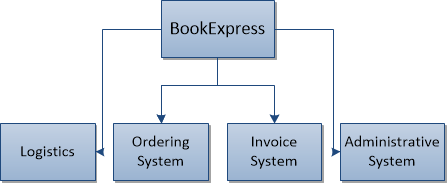
\includegraphics[width=\textwidth]{BookExpress.png}
 \end{center}
 \caption{BookExress}
\end{figure}

\chapter{Software Modules}
\label{sec:modules}
\section{Administrative System}

\begin{figure}[H]
 \begin{center}
  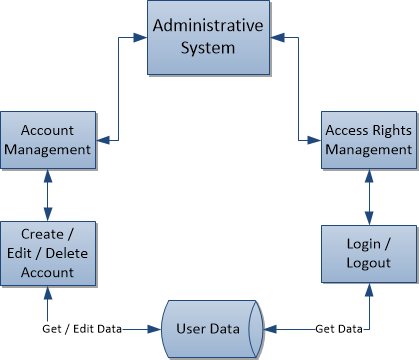
\includegraphics[width=\textwidth]{AdministrativeSystem.png}
 \end{center}
 \caption{Administrative System}
\end{figure}

\subsection{Account Management}

\subsubsection{Create/Edit/Delete Account}

A registered Publisher or BookStore is able to access the Account Management to create, edit or delete its account if he has the rights to do so. The required data is looked up from the User Data database, which returns the requested information.

Editing account information overrides the specific data records in the User Data database only if the changed records are in correct format (i.e. the email address has to has a specific format).

An account is only deletable if the Client hasn't any pending orders which aren't in status "Delivered".

\subsection{Rights Management}

\subsubsection{Login/Logout}

The Rights Management is a security layer for processing the login and logout action performed by any user itself.

Every registered Client or BookExpress employee is able to access the Web Interface. The Login/Logout-Process verifies the entered PIN and password with the User Data database and performs the requested action if the data is correct. The Access Rights Management doesn't need to edit data records of the database but only read them.

If the entered data isn't correct the user gets a notification.

\section{Ordering System}

\begin{figure}[H]
 \begin{center}
  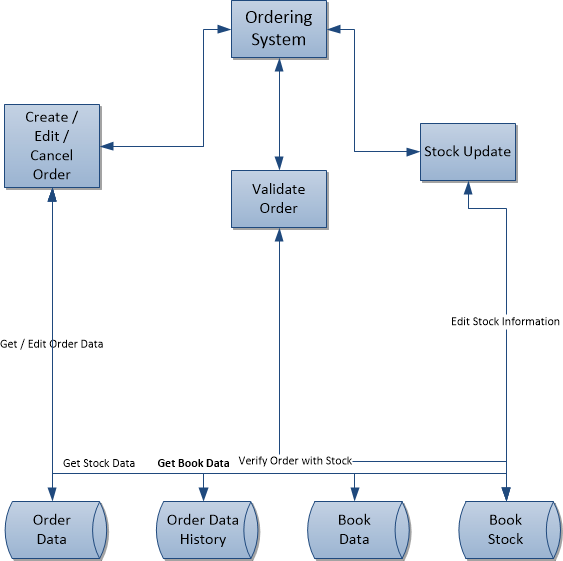
\includegraphics[width=\textwidth]{OrderingSystem.png}
 \end{center}
 \caption{Ordering System}
\end{figure}

\subsection{Order Module/Order Functions}

\subsubsection{Create/Edit/Cancel Order}

For creating an order, a registered client has to be authorised as well. The Edit/Cancel Order process fetches the specific information from the Order Data database. The Create Order process creates a new record in Order Data by accessing information from the Book Data and Book Stock database (User Data is also written into Order Data). The order is set to "Processing" and later on checked for validation.

\subsubsection{Validate Order}

Validate Order checks the status of the requested order and returns "Valid" to the inquirer if the check passed successfully.

\subsubsection{Stock Update}

The Stock Update process runs if either an employee initiates a check or an order was placed by a Client. For every order the system checks the stock for available books and returns a list of recommended books to order.

\section{Logistics System}

\begin{figure}[H]
 \begin{center}
  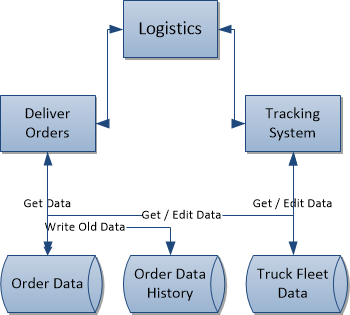
\includegraphics[width=\textwidth]{Logistics.png}
 \end{center}
 \caption{Logistics}
\end{figure}

\subsection{Logistics Functions}

\subsubsection{Deliver Orders}

If the status of an order is "Valid" and the the requested books are currently available in the stock then the the Logistics initiates the delivery process by setting the order status to "Deliver". Therefore the Deliver Orders have to have access to the Order Data database (i.e. get the address of the receiver.)

The Order Data History database saves all processed orders in all states to provide a version history for logging purposes.

\subsubsection{Tracking System}

The Tracking System shows detailed information of the current status of the requested order. If a status is set, the order status is printed. An order can have all possible status defined in the Data Dictionary (see \ref{sec:dd}).

Part of the System is also to receive and edit the dedicated data record in the Truck Fleet Data database. These information are even more precise by showing the current status of the Truck (see  \ref{sec:truckInfo}).

\section{Invoice System}

\begin{figure}[H]
 \begin{center}
  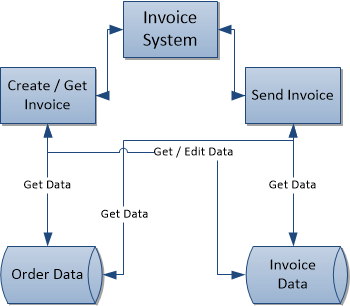
\includegraphics[width=\textwidth]{InvoiceSystem.png}
 \end{center}
 \caption{Invoice System}
\end{figure}

\subsection{Invoice Functions}

The Invoice System handles the invoices which are triggered if the order status is set to "Valid".

\subsubsection{Create/Get Invoice}

The system automatically creates a new invoice which lists all ordered books with title, price, total price and tax.

To process this function the method needs to have access to the Order Data database and the Invoice Data database to request and edit several information.

\subsubsection{Send Invoice}

If the invoice is completed, it is send. The user will get a notification including the invoice and by default the status is set to "Open".

\chapter{Data Dictionary}
\label{sec:dd}
\section{User Data}

\begin{longtable}{p{3.5cm}p{0.5cm}p{8.5cm}}
Client File & = & \{Client Data\} \\
\\
Client Data & = & Client PIN\\
&  & + Address\\
&  & + Correspondent\\
&  & + Contract Data\\
&  & + \{Order\}\\
&  & + \{Invoice\}\\
&  & + (Sales Volume)\\
&  & + Login Data\\
&  & + Account Type\\
& = & Publisher Data\\
& = & Book Store Data\\
\\
Address & = & [Street + Street Number $|$ Post-Office Box]\\
&  & + Name\\
&  & +  (Country Symbol)\\
&  & +  Postal Code\\
&  & + City\\
&  & + Phone Number\\
&  & + (Fax)\\
&  & + Email Address\\
\\
Name & = & Form Of Address\\
&  & + (Title)\\
&  & + Forename\\
&  & + Surname\\
&  & + (Trade Name)\\
& = & Author\\
& = & Publisher\\
& = & Driver\\
\\
Login Data & = & [Client PIN $|$ Employee PIN]\\
&  & + Password \\
\\
Account Type & = & [Book Store $|$ Publisher $|$ Employee]\\
\\
Correspondent & = & Name\\
&  & + (Email)\\
\hfill\\
\caption{Client Data}\\
\end{longtable}


\section{Order Data}

\begin{longtable}{p{3.5cm}p{0.5cm}p{8.5cm}}
Order & = & Order Data\\
\\
Order Data & = & Order PIN\\
&  & + 1\{Article\}\\
&  & + Order Status\\
&  & + Date \\
\\
Order Status & = & [Processing $|$ Valid $|$ Invalid $|$ Logistics $|$ Delivery $|$ Delivered $|$ Canceled] \\
\\
Date & = & Hour\\
&  & + Minute\\
&  & + Day\\
&  & + Month\\
&  & + Year\\
\hfill\\
\caption{Order Data}\\
\end{longtable}

\section{Internal Data}

\subsection{Book Stock}
\begin{longtable}{p{3.5cm}p{0.5cm}p{8.5cm}}
Stock & = & \{Article\} \\
\\
Article & = & Book Data\\
&  & + Amount\\
\\
Book Data & = & [ISBN $|$ UPC $|$ EAN]\\
&  & + 1\{Author\}\\
&  & + Title\\
&  & + Publisher\\
&  & + (Article Cover)\\
&  & + Price\\
&  & + Availability\\
\\
Availability & = & [In Stock $|$ Ordered at Publisher $|$ N/A]\\
\hfill\\
\caption{Book Data}\\
\end{longtable}

\subsection{Truck Information}
\label{sec:truckInfo}
\begin{longtable}{p{3.5cm}p{0.5cm}p{8.5cm}}
Truck Fleet Data & = & Driver\\
&  & + Registration Number\\
&  & + Truck Status \\
\\
Truck Status & = & [Boxing $|$ Parcel Sorting Centre $|$ Delivering $|$ Traffic Jam $|$ Delivered] \\
\hfill\\
\caption{Truck Fleet Data}\\
\end{longtable}

\subsection{User Data}
\begin{longtable}{p{3.5cm}p{0.5cm}p{8.5cm}}
Contract Data & = & Contract PIN\\
& & + Signing Date\\
& & + [Client Data $|$ Employee Data]\\
& & + File On Server\\
\\
Signing Date & = & Day\\
&  & + Month\\
&  & + Year\\
\\
Invoice & = & Client Data\\
&  & + Order\\
&  & + Invoice PIN\\
&  & + Invoice Status\\
\\
Invoice Status & = & [Paid $|$ Open]\\
\hfill\\
\caption{Contract Data}\\
\end{longtable}

\subsection{Employee}

\begin{longtable}{p{3.5cm}p{0.5cm}p{8.5cm}}
Employee File & = & \{Employee Data\}\\
\\
Employee Data & = & Employee PIN\\
&  & + Address\\
&  & + Contract Data\\
&  & + Login Data\\
&  & + Administrator\\
\\
Administrator & = & [True $|$ False]\\
\hfill\\
\caption{Employee Data}\\
\end{longtable}

\begin{longtable}{p{3.5cm}p{0.5cm}p{8.5cm}}
Backup & = &  Client File\\
&  & + Order Data\\
&  & + Stock \\
&  & + Truck Fleet Data\\
&  & + Employee File\\
\hfill\\
\caption{Backup Data}\\
\end{longtable}

\chapter{Mini Specifications}
\section{Internal Product Functions}
\subsection{Employees of "BookExpress"}
\begin{lstlisting}[caption=/PF00/Register Publisher or Book shop (client)]
if (ContractSigned==true) then  
	System.RegisterNewClient;
Registered(Client)=true;
\end{lstlisting}
\begin{lstlisting}[caption=/PF01/Edit client information]
if (Registered(Client)==true) then  
	System.EditClientInfo(Client);
	System.SaveClientInfo(Client;
\end{lstlisting}
\begin{lstlisting}[caption=/PF02/Delete Account]
if ((Registered(Client)==true) and Client.OrderCount==0) then  
	System.DeleteAccount(Client);
	System.SendDeleteNotification(Client);
\end{lstlisting}
\begin{lstlisting}[caption=/PF10/ Client places Order]
if ((Registered(Client)==true) and (Authorised(Client)==true)) then  
	System.ManualOrder(Client, Book);
	Order.Status="Processing";
	System.SendReport(Client);
\end{lstlisting}
\begin{lstlisting}[caption=/PF11/ Validate Order]
if (Order.Status=="Processing") then 
	Order.Check();
	Order.Status="Valid";
	System.SendConfirmation(Client);
\end{lstlisting}
\begin{lstlisting}[caption=/PF12/ Stock Update]
if (Order.Placed(Client)==true or System.InitiateCheck is called) then
	for i=0 to Order.Amount do
		System.StockCheck(Book[i]);
		System.SubmitList(Book[i], (System.StockCheck(Book[i])-Book.AmountOrdered))
\end{lstlisting}
\begin{lstlisting}[caption=/PF13/ Forward Order to Logistics]
if (Order.Status=="Valid" then
	System.SendOrder(Order);
	Order.Status="Logistics";
\end{lstlisting}
\begin{lstlisting}[caption=/PF14/ Deliver Order]
if ((Order.Status=="Valid") and (Book.AmountOrdered <= System.StockCheck(Book))
	Order.Deliver(Client.GetInfo);
	Order.Status="Delivery"
\end{lstlisting}
\begin{lstlisting}[caption=/PF15/ Confirm Delivery]
 Order.Status = Order.TrackingStatus;
\end{lstlisting}
\begin{lstlisting}[caption=/PF16/ BookExpress Order]
 for i=0 to System.StockMax do
 	if System.StockCheck(Book[i])<=System.PredictAmount(Book[i]) then
 	System.OrderBook(Book[i], Book[i].Publisher);
\end{lstlisting}
\begin{lstlisting}[caption=/PF20/ Create Invoice]
if (Order.Status=="Valid") then
	System.NewInvoice();
	for i=0 to Order.Amount do 
		Invoice.Write("Amount:", Book[i].AmountOrdered ,"Book:", Book[i].Title ,"Price:", (Book[i].AmountOrdered * Book[i].Price) )
		Invoice.Total=Invoice.Total + (Book[i].AmountOrdered * Book[i].Price)
		end;
	Invoice.Write("Total:", Invoice.Total)
	Invoice.Write("Tax:", (Invoice.Total * TaxRate));
\end{lstlisting}
\begin{lstlisting}[caption=/PF21/ Send Invoice]
  if (Invoice.Complete==true) then 
  	System.SendInvoice(Invoice);
\end{lstlisting}
\begin{lstlisting}[caption=/PF30/ Backup]
 if (System.Time==2400) then
 	System.RunBackup();
\end{lstlisting}
\begin{lstlisting}[caption=/PF15/ Confirm Delivery]
 Order.Status = Order.TrackingStatus;
\end{lstlisting}

\section{External Product Functions}
\subsection{Book Stores and Publishers}

\begin{lstlisting}[caption=/PF03/ Login]
 if (Registered(Client)) then
 	System.AskPIN();
 	System.AskPassword();
 	if ((System.ValidatePIN()==true) and
 	(System.ValidatePassword()==true)) then
 	System.Login;
\end{lstlisting}

\begin{lstlisting}[caption=/PF04/ Update Account Information]
 if (LoggedIn(Client)) then
 	System.EditData();
 	System.CheckData();
 	System.SaveData();
\end{lstlisting}

\begin{lstlisting}[caption=/PF05/ Logout]
 if (LoggedIn(Client)) then
 	System.ConfirmLogout();
 	System.SessionTerminate();
\end{lstlisting}

\subsection{Book Stores ("Clients")}

\begin{lstlisting}[caption=/PF40/ Search for a Book / Show Catalogue]
 if (LoggedIn(Client)) then
 	System.Search(SearchString)
 	System.ShowResults;
 	Order.Add(Book, Amount);
\end{lstlisting}

\begin{lstlisting}[caption=/PF17/ Book Store Order via Web Interface]
if  (LoggedIn(Client)) then
	Order.Add(Book, Amount);
	System.SubmitOrder(Order);
	Order.Status="Processing";
\end{lstlisting}

\begin{lstlisting}[caption=/PF18/ Change Order]
if  ((Order.Status=="Processing") and (LoggedIn(Client))) then
	System.ShowOrders();
	System.SelectOrder(Order);
	System.EditOrder(Order);
	System.SubmitOrder(Order);
	System.SendChangeNote(Order, Client);
\end{lstlisting}

\begin{lstlisting}[caption=/PF19/ Cancel Order]
if (LoggedIn(Client)) and (Order.Status!=="Delivery"|"Delivered") then
	System.ShowOrders();
	System.SelectOrder(Order);
	Order.Status="Canceled";
\end{lstlisting}

\begin{lstlisting}[caption=/PF50/ Tracking System]
 if (Order.Status!==NULL) then
 System.ShowOrders;
 System.SelectOrder;
 System.Print(Order.Status);
\end{lstlisting}

\subsection{Publishers}

\begin{lstlisting}[caption=/PF60/ Inventory Maintenance]
 if LoggedIn(Publisher) then
 	System.ShowInventory();
 	System.SelectEntry(Entry);
 	System.SaveEntry(Entry);
\end{lstlisting}

\chapter{Appendices}
\printglossaries\addcontentsline{toc}{section}{Glossary}\addcontentsline{toc}{section}{Acronyms}

\listoffigures\addcontentsline{toc}{section}{List of figures}
\listoftables\addcontentsline{toc}{section}{List of tables}

\end{document}